%!TEX encoding = UTF-8 Unicode
\documentclass[a4paper, 14pt, russian]{article}
\usepackage[a4paper]{geometry}
\usepackage[T2A]{fontenc}
\usepackage[utf8]{inputenc}
\usepackage[russian]{babel}
\usepackage{physics}
\usepackage{tcolorbox}
\usepackage{hyperref}
\usepackage{fancyhdr}
\usepackage{indentfirst}
\usepackage{amssymb, amsmath, amsfonts}

\title{Физика полупроводников.\\
        Задача №1}
\author{Куликов Никита}
\date{}

\newcommand{\be}{\begin{equation}}
\newcommand{\ee}{\end{equation}}
\newcommand{\bea}{\begin{equation}\begin{array}}
\newcommand{\eea}{\end{array}\end{equation}}
\newcommand{\mybox}[1]{\fbox{\parbox{1.\textwidth}{#1}}}
\newcommand{\pa}{\partial}
\newcommand{\rot}{\textbf{rot}~}
\renewcommand{\div}{\textbf{div}~}
\renewcommand{\grad}{\textbf{grad}~}
\newcommand{\vep}{\varepsilon}
\newcommand{\ptag}[1]{\tag{\arabic{equation} #1}}
\newcommand{\etag}[1]{\addtocounter{equation}{1}\tag{\arabic{equation} #1}}

\begin{document}
    \maketitle

    \paragraph{Формулировка:} Найти зависимость концентрации
        носителей заряда от температуры $n(T)$ в квантовой яме, имеющей 
        один уровень размерного квантования и параболический закон
        дисперсии:
        \begin{equation}
            \vep(\vec{k}_\perp) = \vep(0) + \frac{\hbar^2 \vec{k}_\perp^2}{2m};
        \end{equation}
        При этом известно, что носители заряда подчиняются статистике
        Ферми-Дирака и имеют уровень Ферми $F$.

    \paragraph{Решение:} Вычислим плотность состояний. Для начала рассмотрим
        интеграл (здесь $S$ - площадь материала):
        \begin{equation}
            \Gamma (\tilde \vep) = \frac{2S}{(2 \pi)^2} \int_{\vep(\vec{k}_\perp) < \tilde \vep} 
                d^2 \vec{k}_\perp = \frac{2S}{(2 \pi)^2}
                \int_{\vep < \tilde \vep} 2 \pi k dk = 
                \frac{4 \pi m S}{(2 \pi \hbar)^2} \int_{\vep < \tilde \vep} 
                d\vep = 
                \left\{\begin{aligned}
                    &  \frac{m S}{\pi \hbar^2} \tilde \vep & \tilde \vep > \vep(0)\\
                    &  0                                 & \tilde \vep < \vep(0)
                \end{aligned}\right.;
        \end{equation}
        В таком случае непосредственно двухмерная плотность состояний (здесь $\Theta$ - функция Хэвисайда):
        \begin{equation}
            g(\vep) = \left. \frac{\pa \Gamma(\tilde \vep)}{\pa \tilde \vep} \right\rvert_{\vep}
                = \underbrace{\frac{mS}{\pi \hbar^2}}_{G} \Theta\big(\vep - \vep(0)\big); 
        \end{equation}
        Теперь будем учитывать статистику Ферми-Дирака:
        \begin{equation}
            f(\vep) = \Big\{1 + \exp\big((\vep - F) / T\big)\Big\}^{-1};
        \end{equation}

        В таком случае среднее число частиц можно вычислить (здесь $\Omega$ - зона Бриллюэна):
        \begin{equation}
            \label{main_formulae}
            \langle n \rangle = \int_\Omega f(\vec{k}_\perp) d^2 \vec{k}_\perp;
            \etag a
        \end{equation}

        Однако, полагая, что уровень Ферми лежит ниже уровня энергии на границе
        Бриллюэна $F \ll \min_{\pa \Omega} \vep$, а также малость температуры в этом смысле
        $F + T \ll \min_{\pa \Omega} \vep$, выражение для концентрации (\ref{main_formulae}) можно
        упростить за счёт хорошей сходимости:
        \begin{equation}
            \langle n \rangle \approx \int_0^{+\infty} g(\vep) f(\vep) d \vep = 
            G \int_{\vep(0)}^{+\infty} \frac{d \vep}{1 + \exp\big((\vep - F) / T \big)}; \ptag b
        \end{equation}
        Этот интеграл можно обезразмерить:
        \begin{equation}
            \langle n \rangle \approx GT \int_{\big(\vep(0)-F\big)/T}^{+\infty} 
            \frac{d\xi}{ 1 + \exp \xi}; \ptag c
        \end{equation}
        В то же время мы знаем первообразную для подынтегральной функции:
        \begin{equation}
            \int \frac{d\xi}{1 + \exp \xi} = \underbrace{\xi - \log(\exp \xi + 1)}_{F(\xi)} + C;
        \end{equation}
        Требуется отметить, что первообразная обращается ноль на бесконечности
        $F(\xi \rightarrow + \infty) \rightarrow -0$, и, что 
        первообразная всюду отрицательна $F(\xi) < 0,~\forall \xi \in \mathbb{R}$. 
        В таком случае концентрация носителей заряда:
        \begin{equation}
            \langle n \rangle \approx GT \bigg(\log\Big(
                \exp\frac{\vep(0) - F}{T} + 1\Big) - \frac{\vep(0) - F}{T}\bigg); \tag{5 c}
        \end{equation}
        Проанализируем зависимость концентрации носителей от температуры. 
        Для простоты положим $G\big(\vep(0) - F\big) = 1,~t = T / \big(\vep(0) - F\big)$.
        В таком случае получим зависимость:
        \begin{equation}
            \langle n \rangle = t \Big(\log\big(\exp(1 / t) + 1\big) - 1 / t\Big);
        \end{equation}
        Построим эту зависимость:
        \begin{center}
            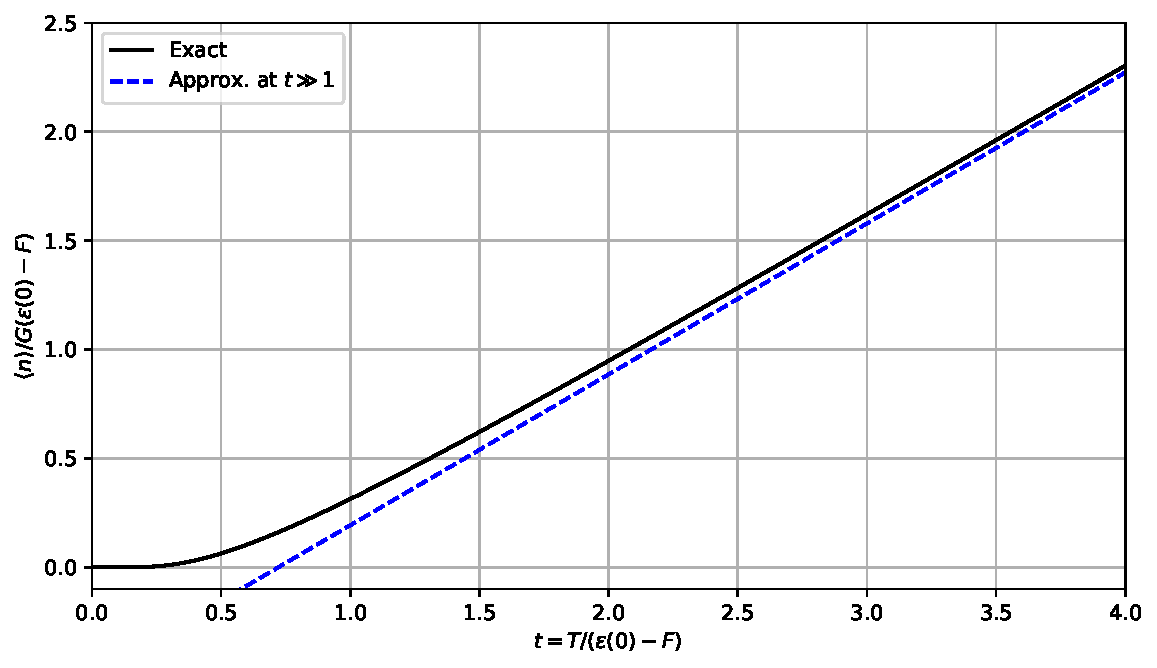
\includegraphics[width = \linewidth]{n_from_t.pdf}
        \end{center}
        На ней можно можно отметить два характерных участка:
        плато в нуле температур и линейный рост при достаточно 
        больших температурах. Начнём с последнего участка $t \gg 1$:
        \begin{multline}
            \langle n \rangle \approx t \Big(\log\big(2 + 1 / t + O(1 / t^2)\big)
                - 1 / t \Big) = t (\log 2 + 1 / 2 t + O(1/ t^2) - 1 / t) =
                \log 2 \cdot  t - 1 / 2 + O(1 / t); 
        \end{multline}
        При близких к нулю температурах $t \rightarrow 0$ разложение принимает 
        другой вид:
        \begin{multline}
            \langle n \rangle = t \bigg(\log\Big(
                \exp(1/t)\big(1 + \exp(-1 / t)\big)\Big) - 1/ t\bigg)
                = t \bigg(1/t + \log\big(1 + \exp(-1 / t)\big)
                - 1 / t \bigg)\\
            \approx t \Big(\exp(-1 / t) + O\big(\exp(-2 / t)\big)\Big) = 
            O\big(t \exp(-1 / t) \big).
        \end{multline}
\end{document}
    
    